


\chapter{Optimal Resource Share Adjustment in Cloud Using Dynamically Tuned Empirical Models} 
\label{ch:optimal_tuning_of_application_resource_shares} 
%\begin{center}
%\textbf{This chapter contains material from Ghanbari et al. \cite{hamoun_ghanbari_feedback-based_2010}}.
%\end{center}

In order to allocate a set of limited resources to a set of applications optimally, there is a need for a model of the application service center. 
A portion of the related work on optimal deployment such as \cite{li_fast_2009,li_performance_2009} assumes that the service center follows an accurate first principle model. They suggest using a filter-based approach such as \cite{zheng-integrated-2011} to estimate the parameters of this model adaptively (i.e. through unsupervised learning).   
However, there is no guarantee that these first principle models accurately represent a service center. It is usually very hard to model all aspects of a service center such as software contention, concurrency, remote calls, a limited amount of memory, and a limited amount of network bandwidth.  

In contrast to the first principle approach, an empirical approach can use a model obtained by regression analysis of application performances. The major problem with present empirical models, is the lack of tuning, based on actual measurement data (e.g. resource utilizations).  
When applications are deployed in a production environment, the models start to lose accuracy. This inaccuracy is mainly because the production conditions are different from the test conditions \footnote{test conditions are used to build the training data sets.}.
 
Our contribution is to increase the accuracy of the empirical models by dynamic tuning using measurement data captured in real-time. We also trace the accuracy increase in the overall performance of the allocation. We investigate if a model built off-line through a nonlinear regression and dynamically tuned through an Extended Kalman Filter, can outperform a model which is not tuned. The other differences between our approach and previous work are in the use of the decomposed models, and in the use of a customized optimization routine to optimize the defined utility functions.   

We show that static non-tuned application models result in a suboptimal allocation decision for some applications leading to missed SLAs. In contrast, we found that the use of dynamically tuned models resulted in more efficient resource allocations, closer achievement of SLAs and better utility. 

The model we develop in this chapter corresponds to a virtualized private data center with limited resources. The unique feature of virtualized data centers when work conservation is enabled is that virtual machines isolate the applications. So, performance of each application can be modelled separately based on allocated resources.
Each application's performance is modelled based on the amount of resources allocated to its VMs. Since the simulator used in this chapter simulates applications with open workloads, we use open queuing network models as a basis of our model.

We assume that the cloud provider only tries to optimize the applications' performances by tuning the amount of resources allocated to the existing fixed set of VMs.  Directly changing ``relative share'' of the allocated resource to each single VM can be done through the hypervisor's scheduler parameters. In addition, the assumption is that the cloud provider can monitor the performance metrics of the applications and thus build models based on the performance metrics and the given resources.
 
Our approach is presented in Figure~\ref{fig:feedback-based-optimization}. 
In this approach, for each application, the cloud provider maintains a dynamically updated performance model. 
A utility function based on a specific service level objective (e.g., response time) is also maintained for each application.    
The performance model for each application is updated periodically based on the measured performance attributes.  The cloud provider then performs a system-wide global optimization (see Section~\ref{sec:optimization-through-subgradient}) using the performance models and determines new resource allocations for each application for the following period. 
\begin{figure}[h]
	\centering
		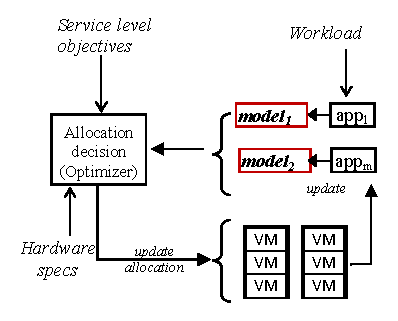
\includegraphics[width=0.45\textwidth]{image/centralized1/image2new}
	\caption[Architecture of the proposed feedback-based optimization approach for private cloud.]{Feedback based optimization of resource shares.} 
	\label{fig:feedback-based-optimization}
\end{figure}

\section{General Definitions} 
\label{sec:general-defs}
In this section, we define the necessary notation used in the specification of the problem. 

\textbf{Applications:} 
To denote applications we use the symbol $c$ since one way to model applications is through classes as defined in a queuing model. Consider applications \texttt{$c_1$},\ldots, \texttt{$c_C$}. Each application runs within one or more VMs and experiences a particular workload.  
For modeling purposes in this chapter, we assume each application experiences an open workload with certain inter-arrival time(s) denoted by $\tau_c$. 
Also, we assume $d_c$ is application $c$'s hardware demand per application request (i.e. the number of CPU cycles for each request to be processed).

\textbf{Hardware Structure:} We assume a private service centre with heterogeneous resources composed of $H$ hosts or physical machines (PM)s represented by the set ${h_0,...,h_H}$. We also assume each host has one resource type. The capacity of the resource of host $h$, is denoted by $\capp_{h}$.   

\textbf{Utility Function:} 
Figure~\ref{fig:service-level-utility-functions} represents a sample service level utility function, where the vertical line indicates the SLA target for the application and utility decreases as the value of the response time approaches the SLA limit.
It is worth noting that any decreasing differentiable quasi-convex function can also be used as a service level utility function, and the only feature of this function is simplicity of the presentation in mathematical form.
The shape of the function, especially after passing the SLA threshold, will affect the behaviour of the optimization algorithm. 
\begin{figure}[h]
	\centering
	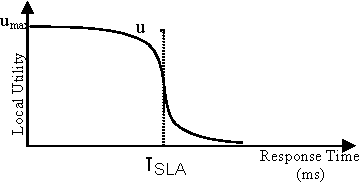
\includegraphics[width=0.45\textwidth]{image/centralized1/image3new}
	\caption[A smooth service level utility function used in a feedback-based optimizer in the private cloud.]{A smooth service level utility function; the vertical line indicates the service level objective of the application (as defined in the SLA).}
	\label{fig:service-level-utility-functions}
\end{figure}

\textbf{Placement:} 
 We consider the VMs of applications which are already deployed on physical machines.
 We specify this deployment through a matrix $\xi$. For each application $c$ and host $h$, if there is a VM allocated to the application on the host, the element $(c,h)$ of matrix $\xi$ is 1 and otherwise  it is 0. 

\textbf{Resource Shares:}
 We represent the allocation of VMs on PMs by a $C \times H$ matrix $\mu^\theta$. Each element $\mu^\theta_{c,h}$ of $\mu^\theta$ denotes a resource allocation defining the percentage of the total resource (i.e. CPU) capacity of the PM $h$ allocated to a running VM of application $c$.  

\section{Problem Formulation}  
\label{sec:contribution2-problem-formulation} 
 Our objective is to maximize a global utility function (sum of application-provided resource-level utility functions $u_c$), subject to a set of capacity constraints which come from the physical layer of the private cloud. 
The optimization problem addressed here can be expressed as follows:
\begin{equation} \label{eq:opt-def}
\begin{split}
\text{given:} 
& \xi_{c,h} \forall c\forall h,
 \tau_c \forall c,l_{\capp,\speedFactor},
 d_{c} \forall c\\
\underset{\mu^\theta}{\text{maximize}} & \sum_{c=0}^{C} u_c(R_c)   \\
\text{subject to: } 
& \sum_{c=0}^{C}{\mu^\theta_{c,h}}<\capp_h \ & \forall h  \\
&  \mu^\theta_{c,h} \geq 0 & \forall h\forall c \\
& R_c=l_{\capp,\speedFactor}(\boldsymbol\mu^\theta_{c},\tau_c,d_{c}) & \forall c \\
& \mu^\theta_{c,h}.\xi_{c,h}=\mu^\theta_{c,h} & \forall c \forall h
\end{split}
\end{equation}
where 
$d_c$ is application $c$'s hardware demand per request and $d_{c}$'s units is the number of CPU cycles.
 
$l$ is a model that maps the application $c$'s resource allocations (i.e. $\boldsymbol\mu^\theta_{c}$) to the service level measure (i.e. response time) of the application, $u_c$ is the local utility function for the application $c$, $\mu^\theta_{c,h}$ represents the allocation of a physical machine $h$ to application $c$. 
In a case study we use a simulator that includes the number of CPU cycles as an input parameter. Each $\mu^\theta_{c,h}$ will be considered to have the unit of million instruction per-second (MIPS). $\boldsymbol\mu^\theta_{c}$ represents the vector of resources allocated to an application $c$ on different hosts. 
The equality constraint $\mu^\theta_{c,h}.\xi_{c,h}=\mu^\theta_{c,h} \  \forall c \forall h$ implies that the only elements of $\mu^\theta_{c,h}$ that need to be optimized are those whose corresponding element in $\xi$ is 1. Other elements of $\theta$ will be considered 0. It is an implication of the first and second inequality constraints that each allocation $\mu^\theta_{c,h}$ is constrained to lie in the interval $[0,\capp_h]$ meaning that an application can maximally get the whole capacity of a PM. The equality constraint relates the response time of each application to the workload intensity, hardware demands, and the given capacities.

Note that the proposed problem solution has a best effort nature, and we treat a service level objective (i.e. target on a specific QoS metric) as a soft constraint by incorporating it into the objective function. 

\section{Selecting an Empirical Model}
A performance model can be used to relate the physical layer specification of a customer's application (e.g. it's given resource shares) and its associated workload to a service level measure (e.g. response time) quantitatively.    
We assume that the response time of each application $c$, can be modelled by the given resources (to VM's) of application $c$ (i.e.$\boldsymbol\mu^\theta_{c}=\{\mu^\theta_{c,1},\dots ,\mu^\theta_{c,H}\}$), the demand of application on the resource types (i.e. here only CPU $d_c$) and the workload of the applications (i.e. $\tau_c$) using the function $l$:
\begin{equation} \label{eq:perf-model_general}
\begin{split}
	%s_c= g(a_{1j},a_{2j},\dots ,a_{nj},{\tau }_c,d_c) \\
	R_c=l_{\capp,\speedFactor}(\boldsymbol\mu^\theta_{c} ,\tau_c,d_{c}) 
	\end{split}
\end{equation} 
 where $\boldsymbol\mu^\theta_{c}$ is a vector of elements $\mu^\theta_{c,h}$, which represent the number of allocated CPU cycles (i.e., measured in MIPS), ${\tau }_c$ denotes the request inter-arrival time in seconds associated with the workload of the application $c$, $d_c$ is application $c$'s hardware demand per request (i.e. the number of CPU cycles for each request to be processed), and $R_c$ is the average response time of the application.

 The nonlinear model is further simplified by using the aggregate resource capacity measure $ \mu^{\theta,\text{Agg}}_c = \sum_{h=1...H}{\mu^\theta_{c,h}}$ instead of the vector of individual values
($\mu^\theta_{c,1},\mu^\theta_{c,2},\dots ,\mu^\theta_{c,H}$):% and replacing $g$
%with $f$:
%\begin{equation} \label{eq:aggregate-cap}
 %\begin{split}
  %s_c= f(\mu^{\theta,\text{Agg}}_c,{\Tau }_c,d_c) \\
  %\text{where}\  \mu^{\theta,\text{Agg}}_c = \sum_{i=1...n}{a_{ij}}       
 %\end{split}
%\end{equation}
  We will assume that all applications deployed on the infrastructure adhere to the same performance model, differing only in the setting
  of various configurable parameters. 
	
	Focusing only on one application called $c$, let $\boldsymbol\beta_{c,t}$ be a vector representing the model coefficients
 and $\left[\mu^{\theta,\text{Agg}}_{c,t},\tau_{c,t},d_{c,t}\right]$ be the measured inputs of the system (i.e. capacities, inter-arrival time and demand) 
at step $t$.  
The model maps $\left[\mu^{\theta,\text{Agg}}_{c,t},\tau_{c,t},d_{c,t}\right]$ and $\boldsymbol\beta_{c,t}$ to the modelled output $R_{c,t}$:
\begin{equation}\label{eq:kalman-model} 
R_{c,t}=f(\left[\mu^{\theta,\text{Agg}}_{c,t},\tau_{c,t},d_{c,t}\right],\boldsymbol\beta_{c,t})
\end{equation}
where $f$ is a runtime approximation of the service level function (or performance model) $l$ defined earlier.

While the function $f$ can take several forms, the online-estimation techniques and optimization method are general and will be considered next in Subsection~\ref{sec:online-model-estimation} and Section~\ref{sec:optimization-through-subgradient}.
% -----------------------------------------------


We considered three parametric forms for function $f$: 
\begin{enumerate}
\item A simple linear model only containing predictor variables\footnote{The model is linear in the parameters $\beta_{c,i}$ not predictor variables.}:\\
$f(\left[\mu^{\theta,\text{Agg}}_{c},\tau_{c},d_{c}\right],\boldsymbol\beta_{c}) = \beta_{c,1} +  \beta_{c,2} d_c - \beta_{c,3} {\tau}_c - \beta_{c,4} \mu^{\theta,\text{Agg}}_c$
\item A more complex linear model with interaction terms \footnote{The interaction term is the product of the subset of our original predictors.} $\mu^{\theta,\text{Agg}}_c \tau_c$ and $\mu^{\theta,\text{Agg}}_c d_c$ to capture the effect of $\mu^{\theta,\text{Agg}}_c$ on response time at different inter-arrival times and demands:\\
$f(\left[\mu^{\theta,\text{Agg}}_{c},\tau_{c},d_{c}\right],\boldsymbol\beta_{c}) = \beta_{c,1} + \beta_{c,2} d_c-\beta_{c,3} {\tau}_c-\beta_{c,4} \mu^{\theta,\text{Agg}}_c-\beta_{c,5} \mu^{\theta,\text{Agg}}_c d_c + \beta_{c,6} \mu^{\theta,\text{Agg}}_c {\tau}_c$
\item  A non-linear model derived from the mean value based formula for open queuing networks ($R=D/(1-\lambda D)$) \cite{lazowska_quantitative_1984} extended to account for capacity:\\
$f(\left[\mu^{\theta,\text{Agg}}_{c},\tau_{c},d_{c}\right],\boldsymbol\beta_{c})=\frac{\beta_{c,1} d_c}{\mu^{\theta,\text{Agg}}_c-\beta_{c,2} d_c/{\tau}_c}$ 
\footnote{This equation can be derived by substituting $D_c$ with
  $d_c/\mu^{\theta,\text{Agg}}_c$ and ${\tau}_c$ with $1/{\tau}_c$ from the base formula, and adding model coefficients (i.e. $\beta_{c,1}$ and
  $\beta_{c,2}$) to compensate for the differences between the system and a pure queuing model. The substitution requires the inter-arrival time
  ($\tau $) to be a homogeneous Poisson process, and inter-arrival
  times ($\tau $) to be exponentially distributed with parameter
  $\tau $ (mean 1/$\tau $).}
\end{enumerate}

To investigate the accuracy of the models, a data-set of the sample application's performance was generated synthetically by invoking the CloudSim simulator \cite{CLOUDSIM2010} using random values for the capacity, demand and the inter-arrival time. Figure~\ref{fig:arrival-rate-effect-on-response-time} presents a partial visualization of the data-set. 
\begin{figure}
	\centering
	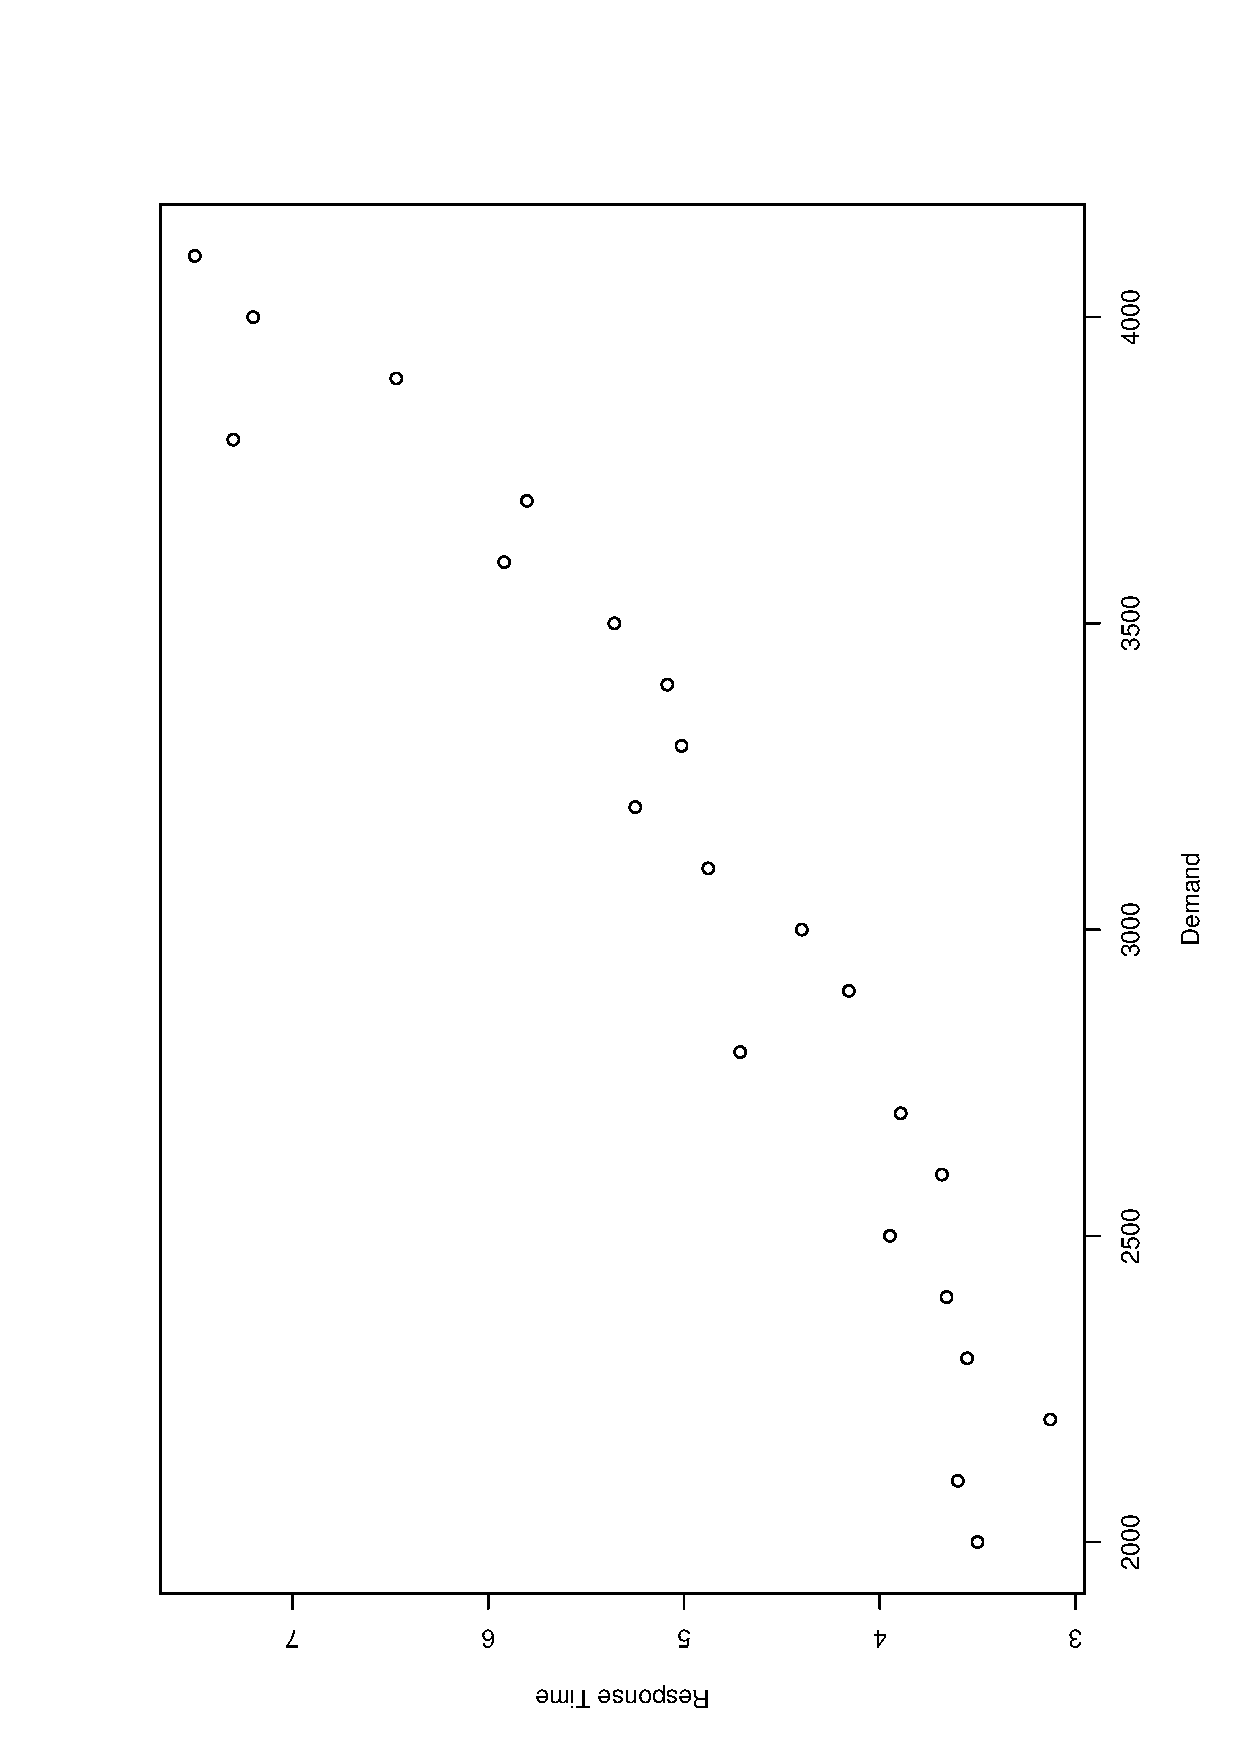
\includegraphics[width=0.45\textwidth,angle=-90,origin=c]{image/centralized1/demand_response_time} \\
	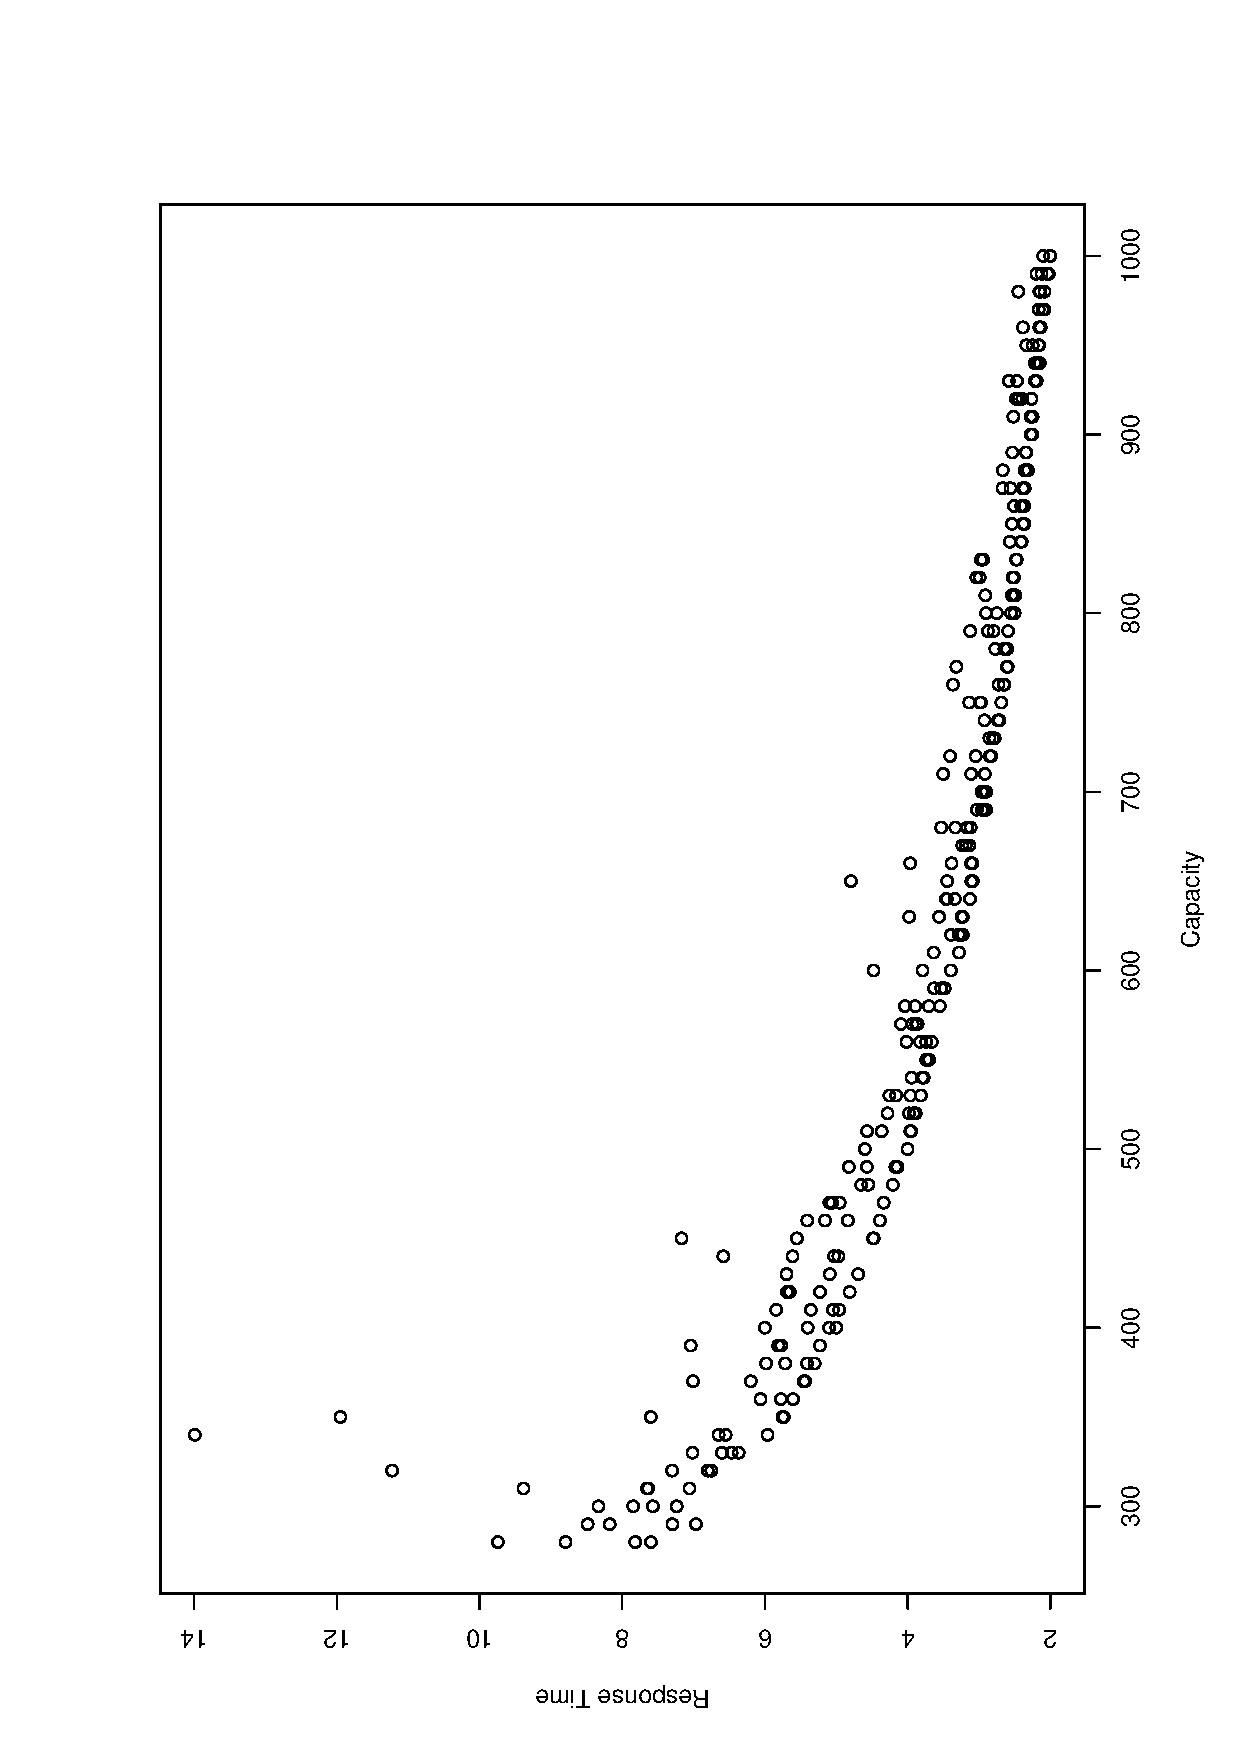
\includegraphics[width=0.45\textwidth,angle=-90,origin=c]{image/centralized1/response_time_capacity}
	\caption[Visualization of pairwise relation between input parameters (capacity,demand) and the response attribute (i.e. response time) for a simulated application.]{Visualization of pairwise relation between input parameters (capacity,demand) and the response attribute (i.e. response time) for a simulated application running on a single VM.}
	\label{fig:arrival-rate-effect-on-response-time}
\end{figure}
A regression analysis was then performed on the resultant data for each model, allowing confidence intervals to be computed for all model parameters.
Usually, the use of a predictor variable is meaningful if its estimated coefficient's confidence interval is far from zero\footnote{There is no proven way for finding if the interval is far enough from 0.}. Moreover, a wide confidence interval usually means lack of accuracy and the need for more data. We formed approximate 95\% confidence intervals for each $\beta_{c,i}$ using mean, standard error, and the normality assumption, to indicate the accuracy and significance of each $\beta_{c,i}$. 
The approximate 95\% confidence intervals for coefficients were quite narrow, and the margins of error were orders of magnitude smaller than the coefficient. This result implies that the amount of data for modeling was adequate.
However, when applying the regression analysis using the linear models, the intervals were very near to zero and coefficients were not significant.
One possible explanation for the lack of significance is that only the fixed portion of the response time (i.e. delay at server) was accounted for in linear models, not the queuing delay which might grow exponentially. 
 The estimated coefficients for the nonlinear model were relatively significant.
As the result of this analysis, the non-linear model's use was validated. 



%\section{Estimation: Online versus Off-line}   
%\label{sec:Modeling-response-time}

% 
\subsection{Online Estimation}
\label{sec:online-model-estimation}

Let $z_{c,t}$ be the measured system output (e.g. response time) at step $t$. 
We further assume that $\beta_{c,t}$ changes according to a random walk:
\begin{equation}
	\boldsymbol\beta_{c,t+1}=\boldsymbol\beta_{c,t}+w_{c,t} \\
\end{equation}
where $w_{c,t}$ represents some Gaussian noise.
A filter maintains the estimate of $\boldsymbol\beta_{c,t}$ and updates it using the linear feedback equation based on new measurements $\left[\mu^{\theta,\text{Agg}}_{c,t},\tau_{c,t},d_{c,t}\right]$ and $z_{c,t}$: 
\begin{equation}\label{eq:kalman-update} 
	\boldsymbol\beta_{c,t} = \boldsymbol\beta_{c,t-1}+ K_{c,t}(z_{c,t} - R_{c,t})
\end{equation}
where $t$ denotes a discrete time index, $K_{c,t}$, the dynamically computed
``Kalman Gain'' matrix and $z_{c,t}-R_{c,t}$ denotes the prediction error\footnote{Note that $R_{c,t}$ was calculated using equation~\ref{eq:kalman-model}.}. With assumptions of system linearity and Gaussian noise, the calculated Kalman gain $K_{c,t}$, is guaranteed to minimize the 
estimation errors for $\boldsymbol\beta_{c,t}$. The updated state will result in a dynamic
model $f(\left[\mu^{\theta,\text{Agg}}_{c,t},\tau_{c,t},d_{c,t}\right],\boldsymbol\beta_{c,t})$ that will be accessed multiple times during optimization cycles. 
Function $f$ and its non-measurable and measurable parameters can have many representations (as shown in Section \ref{sec:case-studies}). 

\section{Optimization}
\label{sec:optimization-through-subgradient}
In this section, the utility maximization problem defined in equation~\ref{eq:opt-def} is solved. Algorithm~\ref{algorithm1} represents a centralized solution for this problem using the primal method.  

The input to the algorithm includes the initial capacities (i.e., $\mu^\theta_0$), the number of iterations during optimization ($k_{\text{max}}$), the performance model ($f_{\boldsymbol\beta_{c,t}}$) and the utility model $u_c$ for each application. 
The output of the algorithm is the optimal allocation matrix ($\mu^\theta_{\text{opt}}$), and maximum utility gained from that allocation ($fp_{best}$) that is obtained iteratively using $k_{\text{max}}$ iterations. )
 \begin{figure} 
\begin{algorithm}[H]  
	\small
	\SetAlgoVlined
	\SetKwInOut{Input}{input}
	\SetKwInOut{Output}{output}
	\SetKwInOut{Initialize}{initialize}
  \SetAlFnt{\tiny}
\footnotesize\Input{
initial capacities $\mu^\theta_0$, 
maximum number of iterations $k_{\text{max}}$, 
performance model $f$,  
utility model $u_c$ forall $c$,
model coefficients $\boldsymbol\beta_{c,t}$ for all $c$}
\Output{optimal allocation $\mu^\theta_{\text{opt}}$, Maximum utility $fp_{\text{best}}$}

initialize: $fp=-\infty$, $fp_{best} =-\infty$, $\mu^\theta=\mu^\theta_0$, $k=0$

\While { $k < k_{\text{max}}$}
{
	compute constraint value $U_i$ for each PM:
	\nllabel{al1-step_1} 
	$U_i(\mu^\theta)=\left(\sum_{c=0}^{C}{\mu^\theta_{c,h}}\right)-\capp_h $

	\If {\text{no constraint is violated:} $max(U_i(\mu^\theta))>0$ //move towards optimum:}
	{
		compute global utility function:
		%using equation~\ref{eq:opt-def}.
		\nllabel{al1-step_2.1} 
		%$U_0 = \sum_{c=0}^{C}  u_c(l_{\capp,\speedFactor}(\boldsymbol\mu^\theta_{c},\tau_c,d_{c})) $
		$U_0 = \sum_{c=0}^{C}  u_c(f(\left[\mu^{\theta,\text{Agg}}_{c,t},\tau_{c,t},d_{c,t}\right],\boldsymbol\beta_{c,t})) $

		record the global maxima: % using equation~\ref{eq-record-global-maxima}.
		\nllabel{al1-step_2.2} 	
		$fp_{\text{best}} \gets max(U_0(\mu^\theta), fp_{\text{best}})$ 

		calculate objective function's subgradient:% using equation~\ref{eq-calculate-objective-subgradient}.
		\nllabel{al1-step_2.3} 
			$g=\partial U_0(\mu^\theta) / \partial \mu^\theta $

		move towards subgradient and the optimum: % using equation:%~\ref{eq-moving-towards-objective-function}.
		\nllabel{al1-step_2.4}			
		$  \mu^\theta \gets \mu^\theta + \alpha g_0$
	}
	\ElseIf{there is some violated constraint}{

	  find most violated constraint using equation:%~\ref{eq-find-most-violated-constraint}.
		\nllabel{al1-step_3.1}
		$m \gets argmax_i(\|U_i(\mu^\theta)\|)$ 
	  \BlankLine

		compute the subgradient value of most violated  constraint as follows:% using equation:%~\ref{eq-calc-subgr-of-most-violated-constraint}.
		\nllabel{al1-step_3.2} 
		% $[(k=m \wedge placement(k,c)=1) \rightarrow (g_m)_{k,c} = 1  ] \wedge   [k \neq m  \rightarrow (g_i)_{k,c} = 0  ]  \  \forall k \forall j$ 
		
		\ \ for each $c$, if $\xi_{m,c}=1$ then  $g_{m,c}\gets 1$ else $g_{m,c}\gets 0$ \nllabel{al1-step_3.2.1}% $\forall c$
		
		\  \ for each $h$ and $c$, if $h \neq m$ then $g_{h,c}\gets 0$   \nllabel{al1-step_3.2.2}%\forall h \forall c$ 
		\BlankLine

		select step size:%based on equation~\ref{eq-step-size-select}.
		\nllabel{al1-step_3.3}
		$\alpha  = (U_i(\mu^\theta_{c,h}) + \epsilon)/(\|g\|^2_2)  $
		\BlankLine

		move away from subgradient and the optimum:
		using equation~\ref{eg:project-subgradient}.\nllabel{al1-step_3.4}
		$\mu^\theta \gets \mu^\theta - \alpha g_i$ 
		\BlankLine
	}
	project each individual variable based on its local constraint:%
	%using equation~\ref{eq-check-local-bound}.
	\nllabel{al1-step_4}  		
	$ \mu^\theta_{c,h} = min(max(\mu^\theta_{c,h},0), \capp_h ) \ \forall h \forall j $ 
	\BlankLine

	$k = k + 1$\; 	
	\BlankLine      
}
$\mu^\theta_{\text{opt}} = \mu^\theta_{c,h}$\;
\caption[A centralized solution for the feedback-based optimization problem using the primal method.]{A centralized solution for the problem using primal method.  
% The equations referred to are presented in Table~\ref{tab:equations}.
}
\normalsize
\label{algorithm1}
\end{algorithm}
\end{figure}

%------------------------------------------
%~\thetb #1
\newcounter{tb}
\newenvironment{tb}[1][]{\refstepcounter{tb}}

\begin{tb}\label{eq-compute-PM-constraint}\end{tb} 
\begin{tb}\label{eq-compute-global-utililty-function}\end{tb}  
\begin{tb}\label{eq-record-global-maxima}\end{tb} 
\begin{tb}\label{eq-calculate-objective-subgradient}\end{tb} 
\begin{tb}\label{eq-moving-towards-objective-function}\end{tb} 
\begin{tb}\label{eg:project-subgradient}\end{tb} 
\begin{tb}\label{eq-find-most-violated-constraint}\end{tb} 
\begin{tb}\label{eq-calc-subgr-of-most-violated-constraint}\end{tb} 
\begin{tb}\label{eq-step-size-select}\end{tb} 
\begin{tb}\label{eq-check-local-bound}\end{tb} 
  % -----------------------------------
 The algorithm performs $k_{\text{max}}$ iterations. In each iteration it does the
  following:

\begin{enumerate}

\item  Computes the constraint values (a constraint is violated if its value is less than 0). A constraint for each physical machine (PM) is the sum of all resources given to VMs deployed on that PM minus the PM's total capacity (step 1).
\item  If the current allocation point is feasible (i.e. no constraint is violated) the algorithm re-calculates the objective function value $U_0$ using the current allocation ($\mu^{\theta,\text{Agg}}$), performance model $f$ from equation~\ref{eq:perf-model_general}, and utility model $u_j$ defined by the administrator (step \ref{al1-step_2.1} ). 
\item If the objective value was greater than the currently reached maxima, it would be recorded (step \ref{al1-step_2.2}).
\item Then the algorithm calculates the objective subgradient using numerical differentiation (i.e. solving the current performance model multiple times for near values of the current point) as if the problem were unconstrained (step \ref{al1-step_2.3}).
\item Finally, a new allocation matrix is calculated, by moving towards the objective function subgradient with a fixed step size (optimality update, step \ref{al1-step_2.4}).
\item If the current allocation point is infeasible the algorithm chooses the most violated constraint\footnote{Actually, this can be any violated constraint.} (step \ref{al1-step_3.1}).
\item Then the algorithm projects the current point onto the set (half-space) of points that satisfy that inequality constraint. 
 Projection is done by moving towards the opposite direction of the constraint function subgradient, $g_i$ (step \ref{al1-step_3.4}).
% while the subgradiet $g_i$ of a constraint $i$ is defined as follows (see step \ref{al1-step_3.2}): 
%\begin{equation}\label{eq:calc-subgr-of-most-violated-constraint}
%\begin{split}
%g_{ij}=(\partial U_i(a)/(\partial a_{ij}))_{ij} = \\
%\left\{ 
			%\begin{array}{cc}
				%0 & placement(i,j)\neq i \\ 
				%1 & placement(i,j)=i 
			%\end{array}
		%\right.
%\end{split}
%\end{equation}
 The sub-steps \ref{al1-step_3.2.1} and \ref{al1-step_3.2.2} assert that, since each constraint is sum of allocated capacity for each VM, $\partial U_i(x)/\partial x$ is a matrix with same dimensions as $x$ (with 1 in each element that affects the constraint). For example if $f(x)_i=x_1-6$ then $\partial f(x)_i/\partial [x1,x2]=[1,0]$. 
% \footnote{$U_i(a)$  changes proportionally with respect to the capacity change $a_{ij}$ of application $j$ 
%(i.e.  ${(\partial U_i(a)/\partial a_{ij})}_{ij}=1$  only if VM of app $j$ is placed on $PM_i$ ). 
%If a VM of application $j$ is not placed on $PM_i$ , $U_i(a)$ will not change with respect to change of
% $a_{ij}$ and thus  ${(\partial U_i(a)/\partial a_{ij})}_{ij}=0$ .}. 

\item The step size is calculated in step \ref{al1-step_3.3}. While $\epsilon>0$ is a tolerance which can take-on different values (e.g. $10^{-3}$,$10^{-2}$, etc.). 

\item  Finally we check that each allocated capacity is feasible and longer than the local bounds (step \ref{al1-step_4}):
where $lb$ is the lower bound and $ub$ is the upper bounds.

\end{enumerate}


%----------------------------------

 For clarity, the equations referenced by the algorithm are listed in Table~\ref{tab:equations}. 
\begin{table*}[h]
\begin{tabular*}{1.0\textwidth}{p{.02\textwidth}>{$\displaystyle}p{.86\textwidth}<{$} }
 %\toprule
  % \footnotesize \text{Num- } & \text{Equation}  \\
\toprule
1 &  U_i(A)=\left(\sum_{c=0}^{C}{\mu^\theta_{c,h}}\right)-\capp_h \\
2 & U_0 = \sum_{c=0}^{C}  u_c( f(\left[\mu^{\theta,\text{Agg}}_{c,t},\tau_{c,t},d_{c,t}\right],\boldsymbol\beta_{c,t}))  \\
3 & fp_{\text{best}} \gets max(U_0(\mu^\theta), fp_{\text{best}}) \\
4 & g=\partial U_0(\mu^\theta) / \partial \mu^\theta \\
5 &  \mu^\theta \gets \mu^\theta + \alpha g_0 \\
6 & \mu^\theta \gets \mu^\theta - \alpha g_i \\
7 & i \gets argmax_i(\|U_i(\mu^\theta)\|) \\
8 &  [(k=i \wedge \xi_{k,c}=1) \rightarrow (g_i)_{k,c} = 1  ] \wedge   [k \neq i  \rightarrow (g_i)_{k,c} = 0  ]  \  \forall k \forall j  \\
9 & \alpha  = (U_i(A) + \epsilon)/(\|g\|^2_2)  \\
10 & \mu^\theta_{c,h} = min(max(\mu^\theta_{c,h},0), \capp_h ) \ \forall h \forall c \\
\bottomrule
\end{tabular*}
\caption{Equations referenced by Algorithm~\ref{algorithm1}.}
\label{tab:equations}
\end{table*} 
To describe the equations briefly: 
Equation 1 states that the value of the constraint\footnote{Value of a constraint here refers to the degree that the constraint is satisfied (positive values) or violated (negative values).} for each $PM_i$ ($i>0$) is the sum of all resources given to VMs deployed on that PM minus the PM's total capacity.
Equation 2 gives the global utility function $U_0$.
Formula 3 is the incremental recording of objective value.
Equation 4 is used to calculate the objective subgradient as if the problem were unconstrained.
Equation 5 indicates moving towards the objective function subgradient with a fixed step size (i.e. optimality update).
Equation 6 is projecting the current point onto the set of points that satisfy the inequality constraint $i$.
Equation 7 denotes choosing the most violated constraint. 
Equation 8 is calculating the subgradient $g_i$ of a constraint $i$ (i.e. $\partial U_i(\mu^\theta)/\partial \mu^\theta$) while $i>0$. 
Equation 9 calculates the step size in the feasibility update, while $\epsilon>0$ is a tolerance and set to $10^{-3}$. 
Equation 10 checks that each allocated capacity is feasible and is between the local bounds. 

To illustrate the optimization algorithm, we consider a pre-built model of one physical machine hosting two applications, each running on a single VM. Both applications have CPU demands of 5100 and 4100 MIPS per request respectively, and response time thresholds of 16 and 7 respectively. The request inter-arrival time of both applications is 22 seconds, and their $u_{\text{max}}$ is 10.  A single PM's CPU, which is used to host these applications, has a total capacity of 1200 MIPS.
 Assumed capacities $\mu^\theta_{11}$ and $\mu^\theta_{21}$ are the CPU allocation for VM1 and VM2. Figure~\ref{fig:sample-config-space-for-subgradient-optimization} shows the entire configuration space over these capacity allocations, constrained by inequalities:
 $\mu^\theta_{11}+\mu^\theta_{21}<1200$, $\mu^\theta_{11}>280$, and $\mu^\theta_{21}>280$.
Note how the optimizer climbs up the global utility function, hits the constraint (i.e., $\mu^\theta_{11}+\mu^\theta_{21}<1200$) then continues to climb and reach the maximum.

\begin{figure}[h]
	\centering
		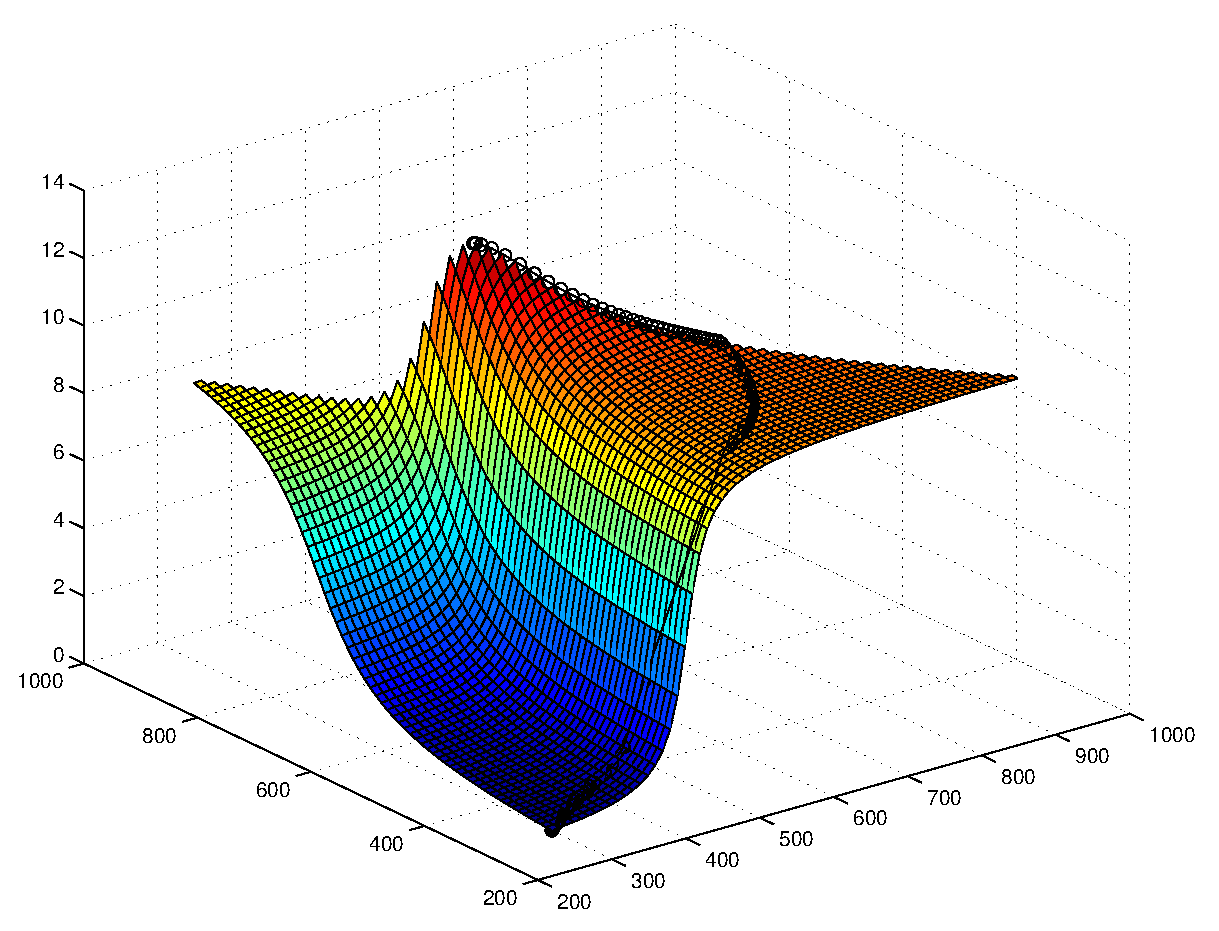
\includegraphics[width=0.8\textwidth]{image/centralized1/twoVM_1PM_optimality}
		\caption{One sample run of subgradient optimization algorithm, finding the
		maximum utility using variations in capacity.}   
	\label{fig:sample-config-space-for-subgradient-optimization}
\end{figure} 


\section{Case Studies}
\label{sec:case-studies}
For the case studies, we simulated a private cloud with the CloudSim~\cite{CLOUDSIM2010} simulator. 
We further considered a very simple local utility function for applications:
\begin{equation} \label{eq:local-utility-formula}
u_c = u_{{\text{max}}_c}\cdot\frac{\left(\arctan(r_{\text{thr}_c}-r_c)+ \pi/2\right)}{\pi} 
\end{equation}
where $u_{{\text{max}}_c}$ denotes the maximum possible utility, $r_{\text{thr}_c}$ denotes the SLA limit (in terms of the minimum response time) and
$r_c$ denotes the actual response time.

\subsection{Case Study One}
\label{sec:case-study-test-simple-deploy}
 % In this section, we study a simulated example to illustrate the applicability of the proposed approach. 
Consider a small cloud configuration with three applications (\texttt{app1}, \texttt{app2}, \texttt{app3}) deployed on two PMs with the following placement matrix:
\[ \xi^T= 
  \left( \begin{array}{ccc}
  1 & 1 & 0 \\
  0 & 1 & 1 \\
\end{array} \right)\] 
That is, \texttt{app1} is deployed on PM1, \texttt{app3} is deployed on PM2, and \texttt{app2} uses both PMs by having a VM on each.

Both of the PMs have single core CPUs with each core having the processing speed of 1200 MIPS and 2 GB of ram. The VMs for applications are identical, each with image size of 1 GB, ram of 512 MB, and bandwidth of 1 GB.

The CPU resource share for each VM is initialized to 280 MIPS but will be adjusted by the optimizer. The applications have workloads with mean CPU demand per request of 4100, 5700 and 500 MIPS respectively. For \texttt{app2}, the load is distributed evenly between the two VMs. We chose the arrival-rates of applications, from the FIFA '98 workload~\cite{arlitt_workload_2000}. The inter-arrival times of requests for all dynamic pages were extracted, on a per-minute basis, from the first six hours of day 21 of FIFA98 workload. To incorporate the time-of-a-day effect, we divided the workload into three 2-hour periods and applied each as an application workload (see Figure \ref{fig:7}). Moreover, we multiplied inter-arrival times of applications by 14, 11 and 8 respectively.
The third application is more transactional in nature (i.e. lower demand and higher inter-arrival time) while the first two are characterized as batch-like.

The utility functions are defined for each application based on equation~\ref{eq:local-utility-formula} with the following parameters for each application:
\begin{align*} \textbf{R}^\text{SLA} = & [15,16,2] \\
 \textbf{u}_{\text{max}} = & [20,10,5]      \end{align*}

For each of 120 samples of inter-arrival times, we submit 20 transactions for each application in the simulator. 
We ran the experiment twice. One run used the static model with the coefficients computed off line as mentioned above.  The second run used the same model but tuned at runtime.
In the case of the tuned model, the new measurements obtained from the simulator (e.g. response times) were used to update the dynamic model's coefficients.  In the case of a static model, the optimizer used the model obtained through regression analysis as-is and no tuning was performed. The optimizer then recalculated the new resource allocations, passed the new allocation vector to actuators to apply it to the system. 

Figure~\ref{fig:case-study1} presents the results. The use of static non-tuned models by the
applications results in a bad allocation decision for \texttt{app2} and leads to failure in meeting app2's SLA (see Figure~\ref{fig:3}).
This results in achieving a suboptimal utility (see Figure\ref{fig:1}).  
In contrast, using dynamic models results in more efficient resource allocations being made, better commitment to SLAs for \texttt{app2} (see Figure~\ref{fig:4}) and better utility (Figure\ref{fig:2}). Figure \ref{fig:5} and \ref{fig:6} represent the allocated capacity to applications over time in case of dynamic models; \ref{fig:5} is for PM1 and \ref{fig:6} is for PM2.     
 
\begin{figure}
	\centering
 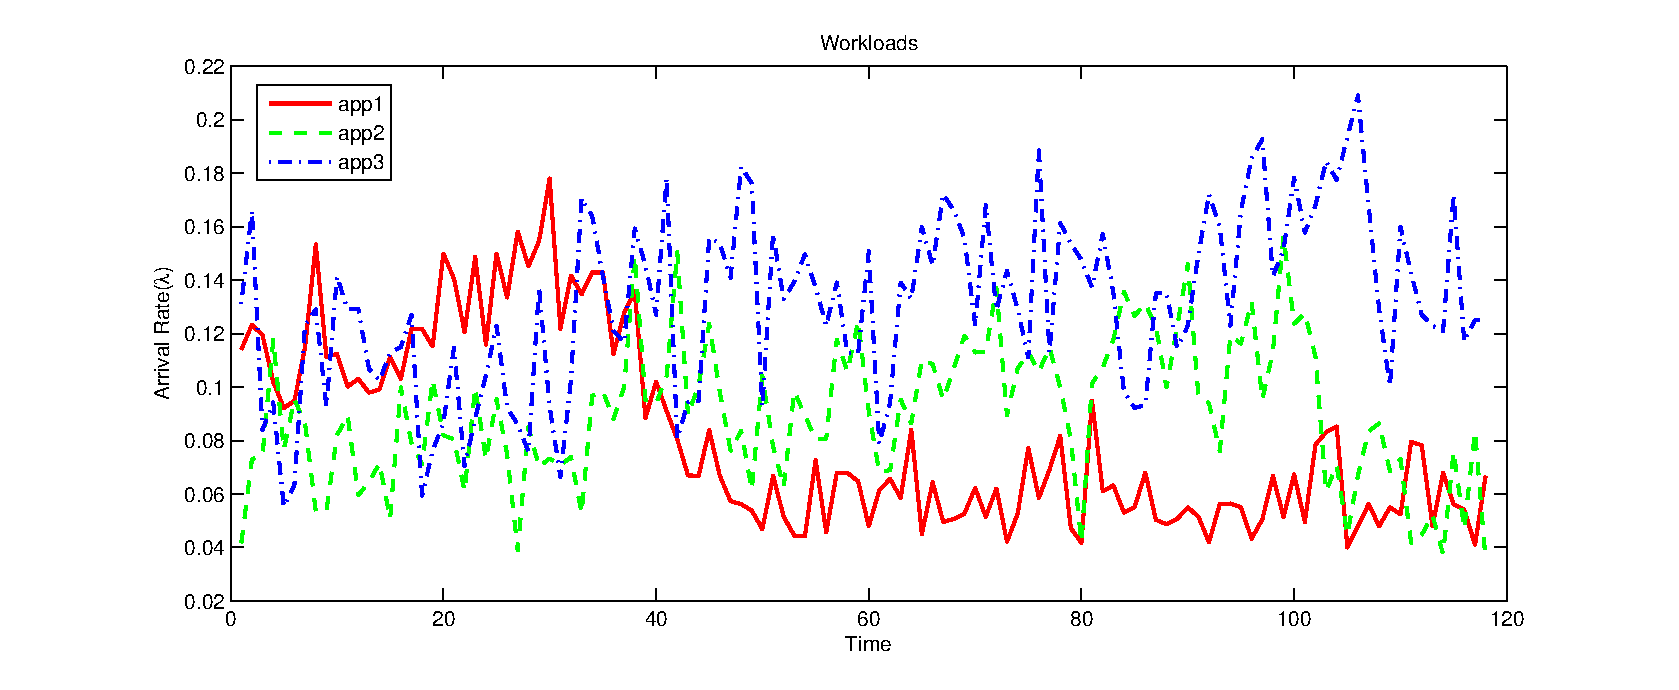
\includegraphics[width=1\textwidth]{image/centralized1/exp_simple_deploy-workload} 
\caption[A sample workload for the applications in a private cloud.]{The workload of applications. }
\label{fig:7}
\end{figure}

\begin{figure}
	\centering
\subfloat[][]{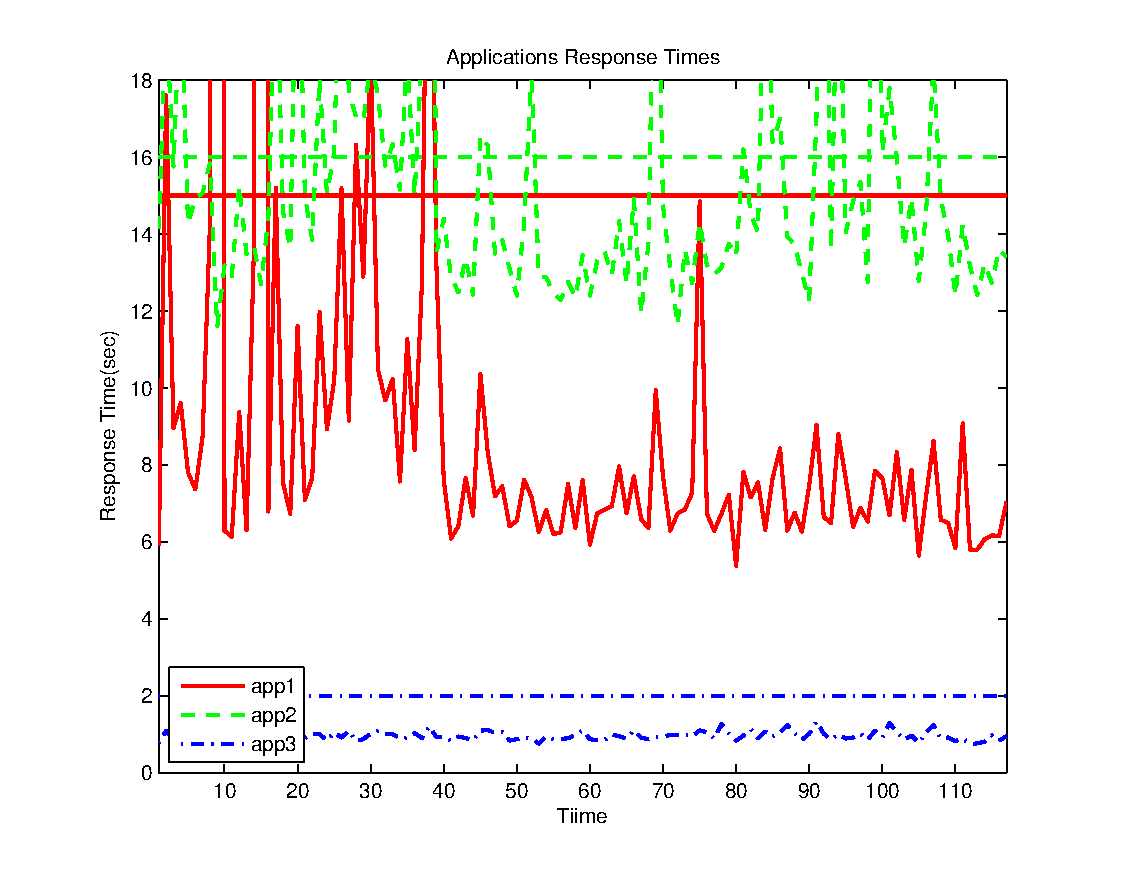
\includegraphics[width=0.5\textwidth]{image/centralized1/exp_simple_deploy-response_time}
\label{fig:3}}% (c) 
\subfloat[][]{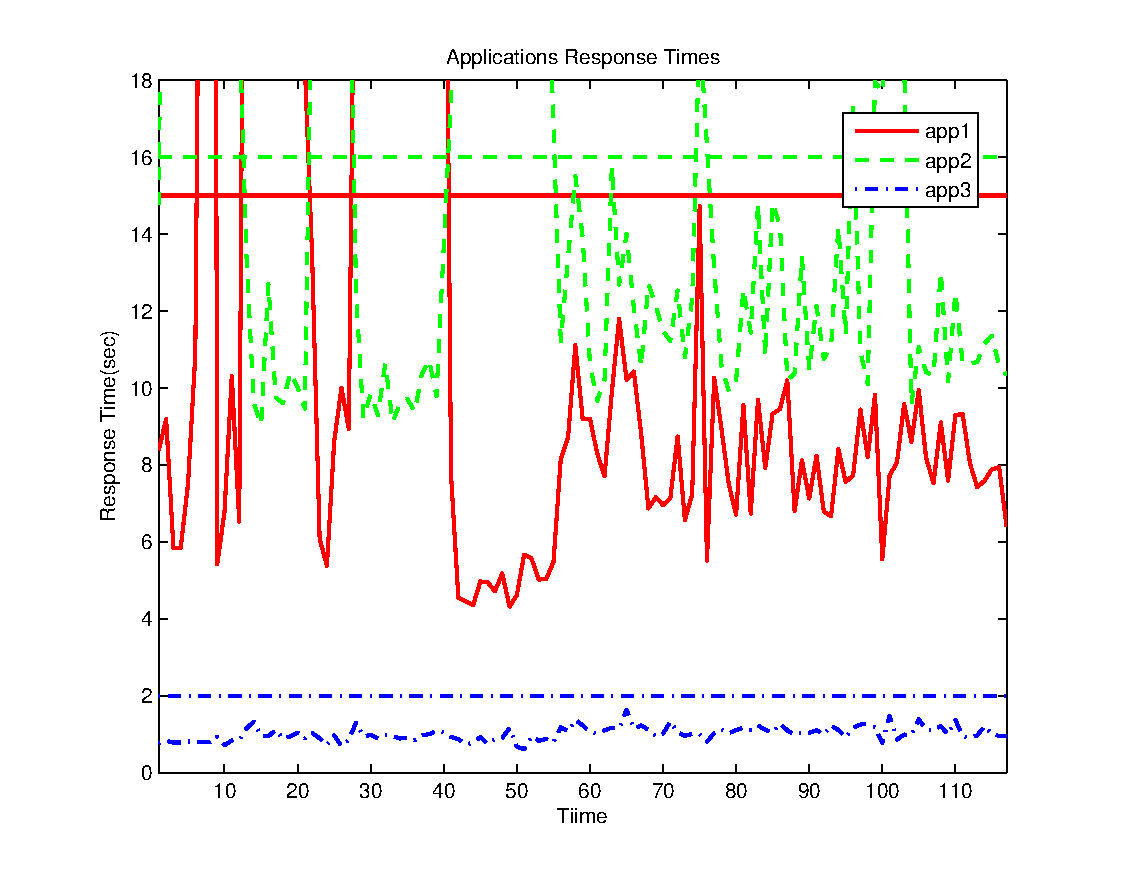
\includegraphics[width=0.5\textwidth]{image/centralized1/exp_simple_deploy_track-response_time}\label{fig:4}}% (d)
\caption[The achieved response time of applications in the simulated private cloud.]{The response time of applications together with SLA response times for \protect\subref{fig:3} static and \protect\subref{fig:4} dynamic models.}
\end{figure}

\begin{figure}
	\centering
\subfloat[][]{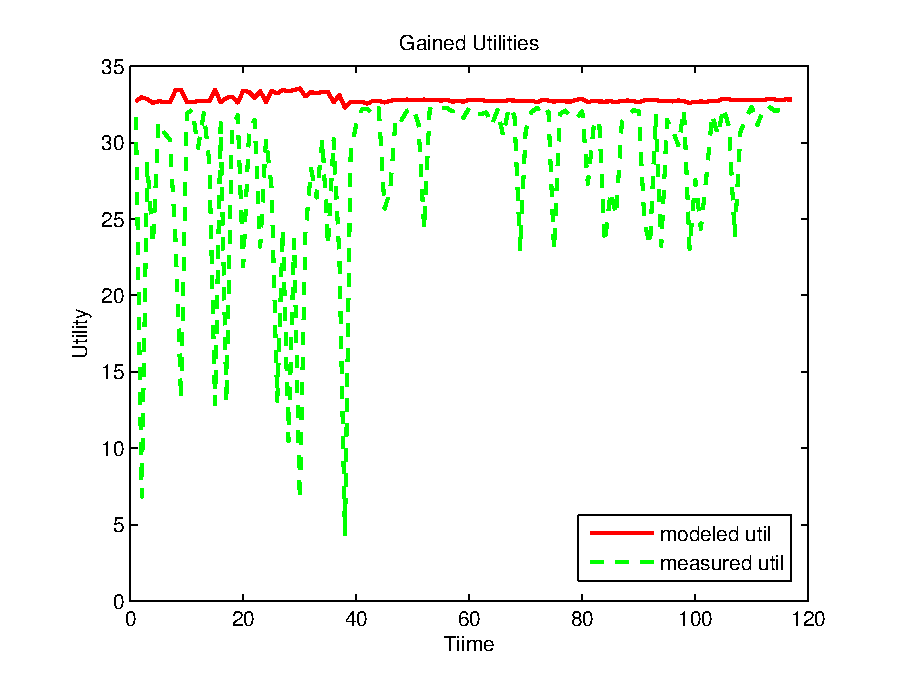
\includegraphics[width=0.5\textwidth]{image/centralized1/exp_simple_deploy-utility} 	
\label{fig:1}}% (a)
 \subfloat[][]{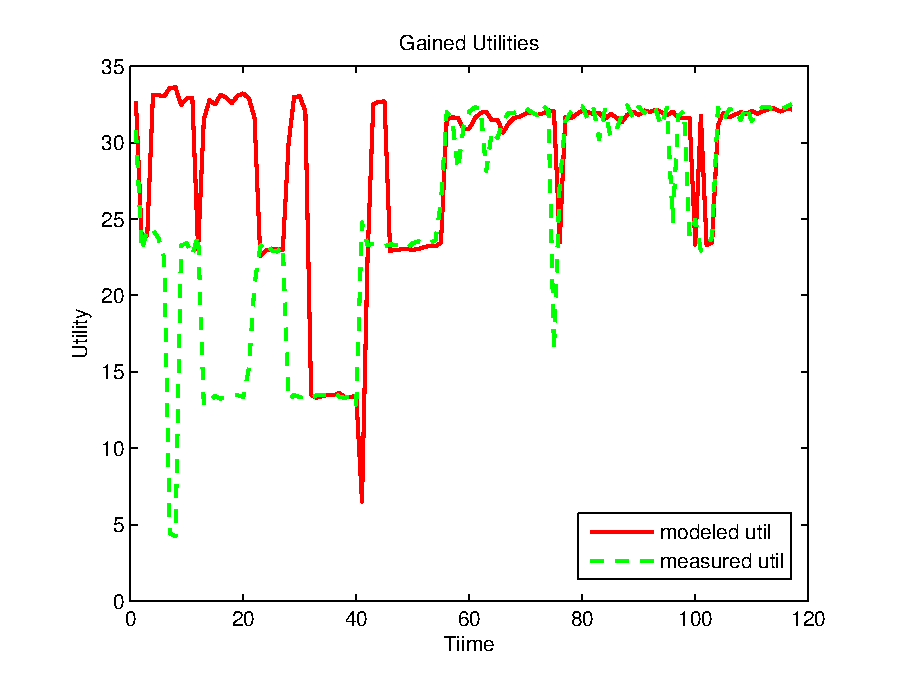
\includegraphics[width=0.5\textwidth]{image/centralized1/exp_simple_deploy_track-utility}\label{fig:2}}% (b) 
\caption[The measured and modelled gained global utility using static and dynamic models over time.]{The measured and modelled	gained global utility using \protect\subref{fig:1} static and \protect\subref{fig:2} dynamic models over time. } 
\end{figure}

\begin{figure}
	\centering
\subfloat[][]{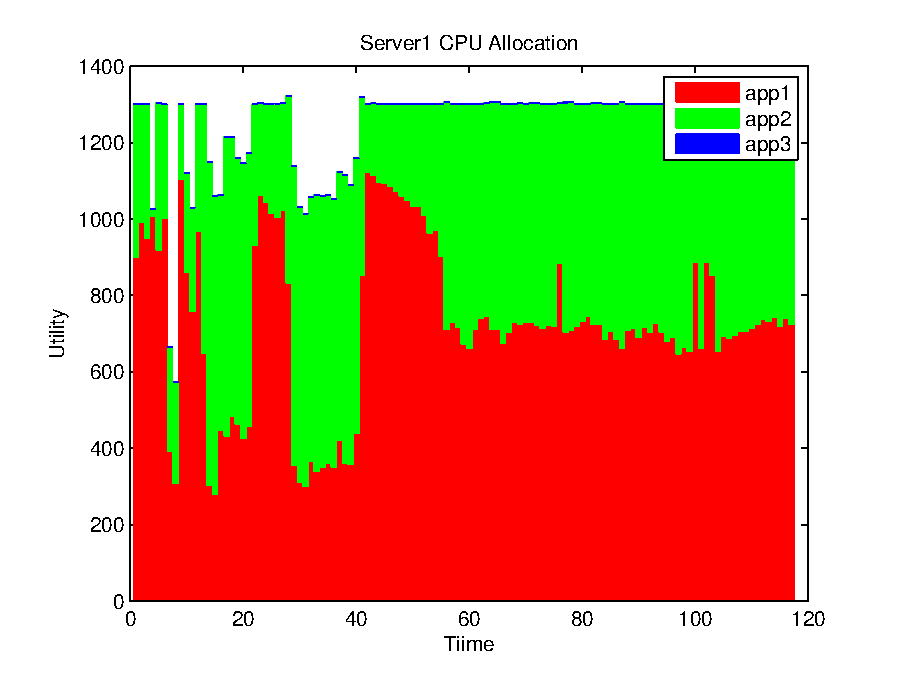
\includegraphics[width=0.5\textwidth]{image/centralized1/exp_simple_deploy_track-server1_cpu}\label{fig:5}}% (e) 
\subfloat[][]{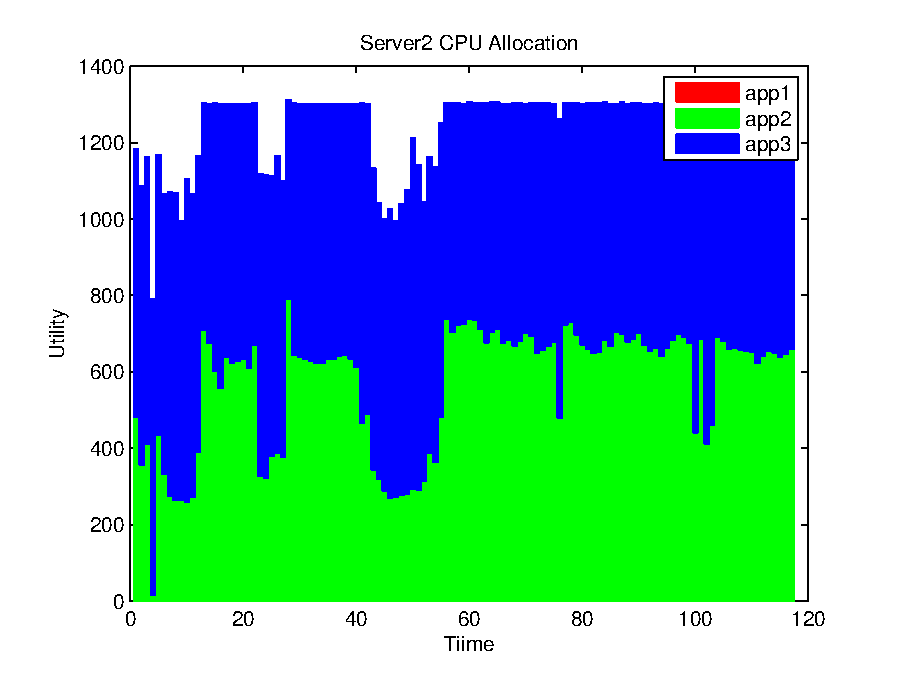
\includegraphics[width=0.5\textwidth]{image/centralized1/exp_simple_deploy_track-server2_cpu}\label{fig:6}}% (f) 
\caption[The allocated capacity to applications over time on server one and server two respectively using dynamic models.]{The allocated capacity to applications over time on \protect\subref{fig:5} server one and \protect\subref{fig:6} server two, using dynamic models. }
	\label{fig:case-study1}
 \end{figure}

% 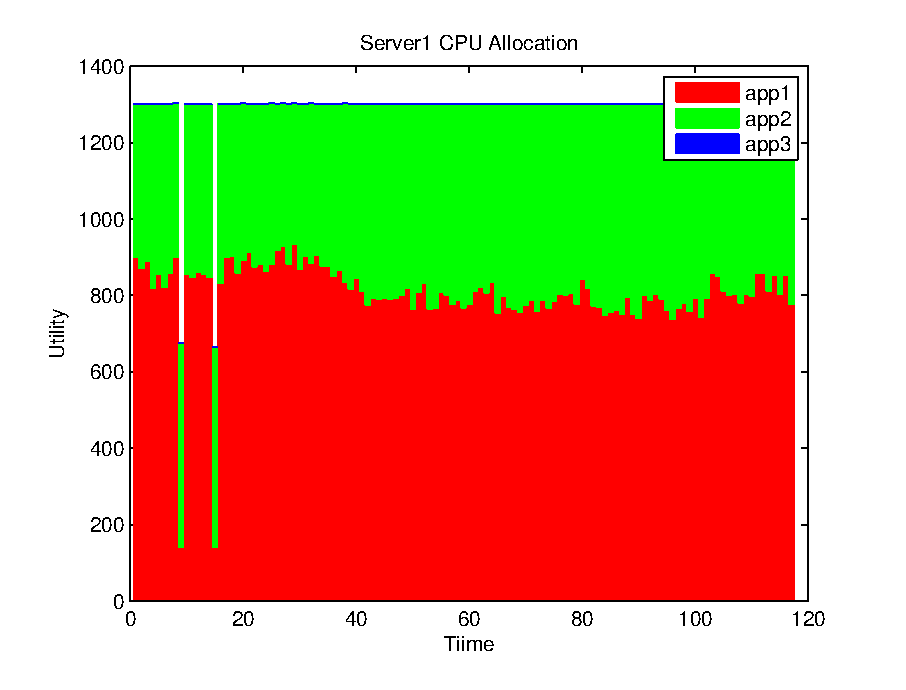
\includegraphics[width=0.45\textwidth]{exp_simple_deploy-server1_cpu}
% 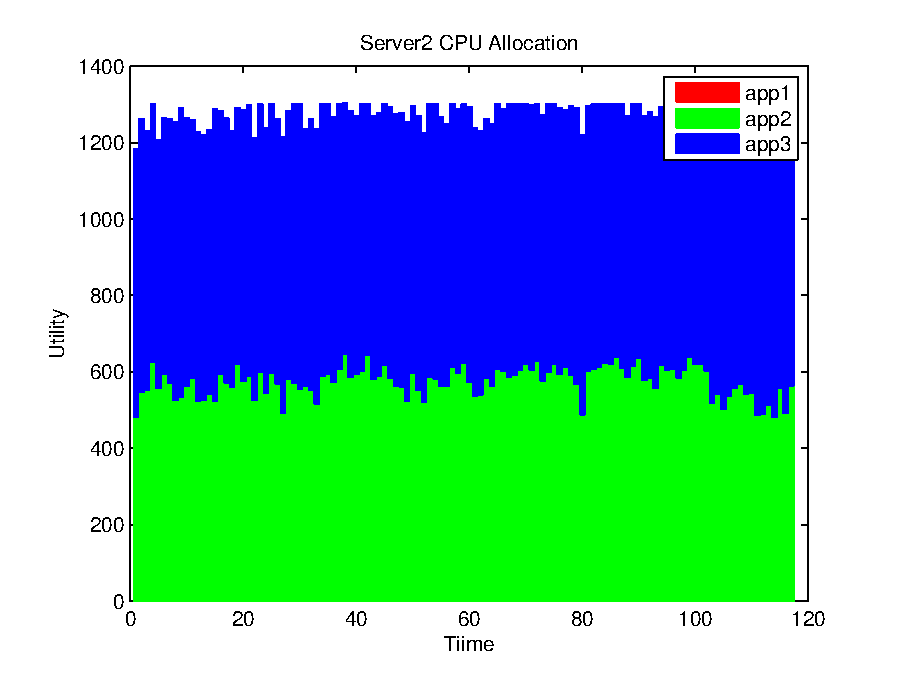
\includegraphics[width=0.45\textwidth]{exp_simple_deploy-server2_cpu}

\subsection{Case Study Two}
\label{sec:case-study2} 

The second case study was performed to demonstrate the ability of our approach to update the resource shares in a way that compensates for the additional workload. Ten applications were deployed on seven PMs.  VMs were assigned randomly to PMs.  All application workloads were set to have an inter-arrival time of 40 seconds except \texttt{app1} whose workload was monotonically increased (i.e., inter-arrival time was decreased from 40 to seven seconds).
\begin{figure}[h]
	\centering
	\subfloat[][]{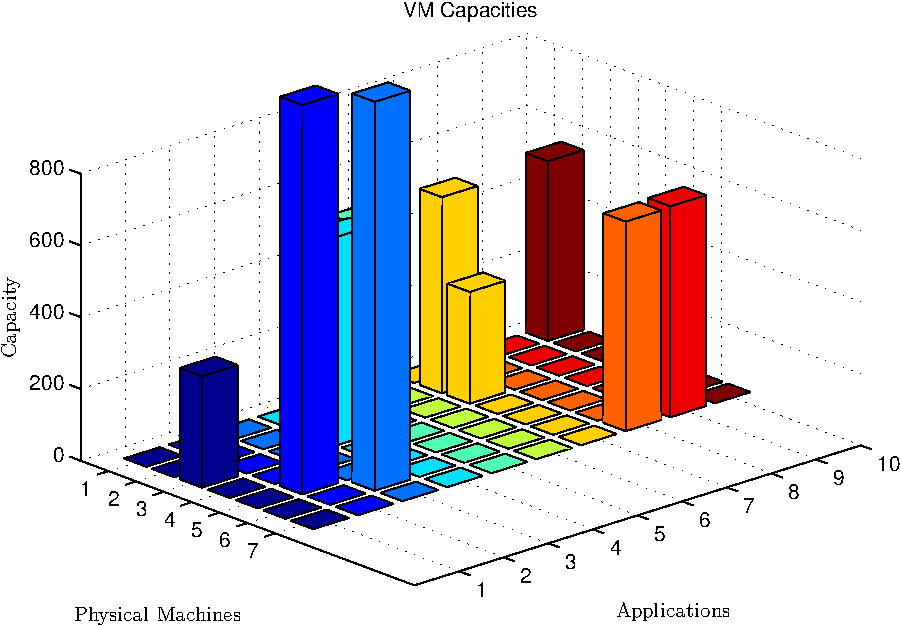
\includegraphics[width=0.5\textwidth]{image/centralized1/first_step}~\label{fig:case-study2-a}}
	\qquad
	\subfloat[][]{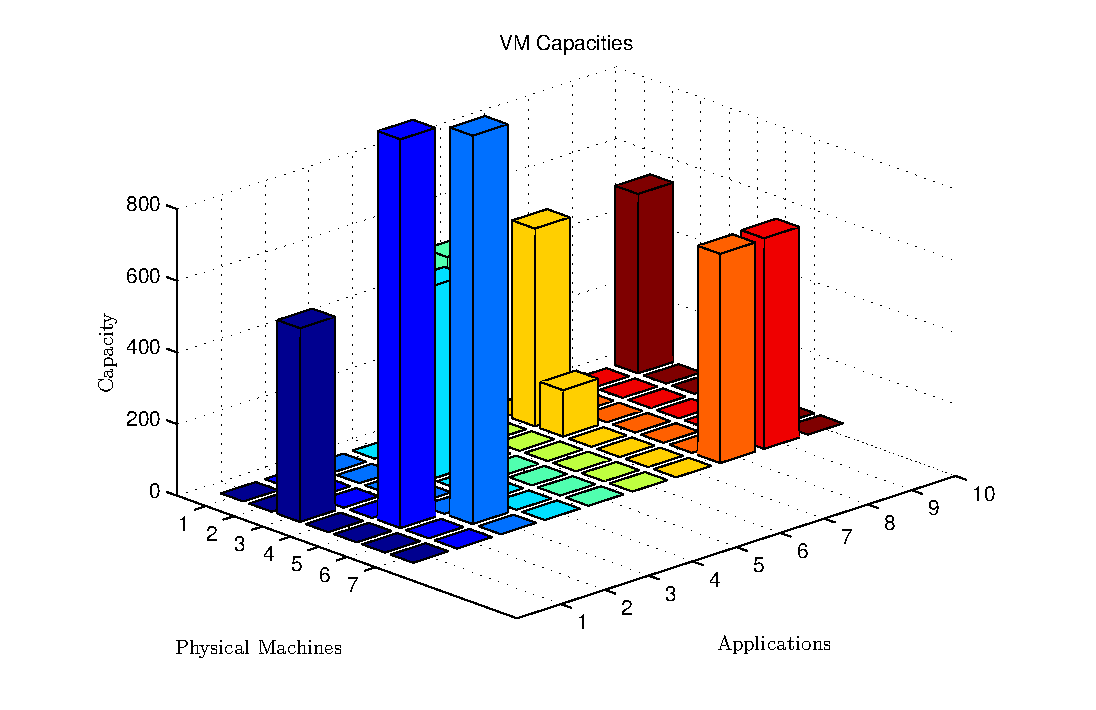
\includegraphics[width=0.5\textwidth]{image/centralized1/last_step}~\label{fig:case-study2-b}} %
	\caption[A snapshot of resource allocation both before and after an increase in the workload is detected.]
	{A snapshot of resource allocation both (a) before and (b) after an increase in the workload is detected.}	\label{fig:case-study2} 
\end{figure}
Figure~\ref{fig:case-study2} presents both before (a) and after (b) snapshots of resource allocations.  Note that both \texttt{app1} (dark blue) and \texttt{app7} (yellow) are resident on the same PM.  Initially, \texttt{app1} is allocated approximately 300 MIPS while \texttt{app7} is allocated approximately 310 MIPS. After the increase in the workload, \texttt{app1} is allocated approximately 510 MIPS while \texttt{app7} is allocated approximately 100 MIPS.

%\subsection{Assessing the Scalability}
 %In addition to the experiments performed in cases studies one and two, the relationship between the number of simulated VMs and the optimization time per step was also considered and a non-linear but polynomial relation was observed (see Figure \ref{fig:scalability}). 
	%\centering
	  %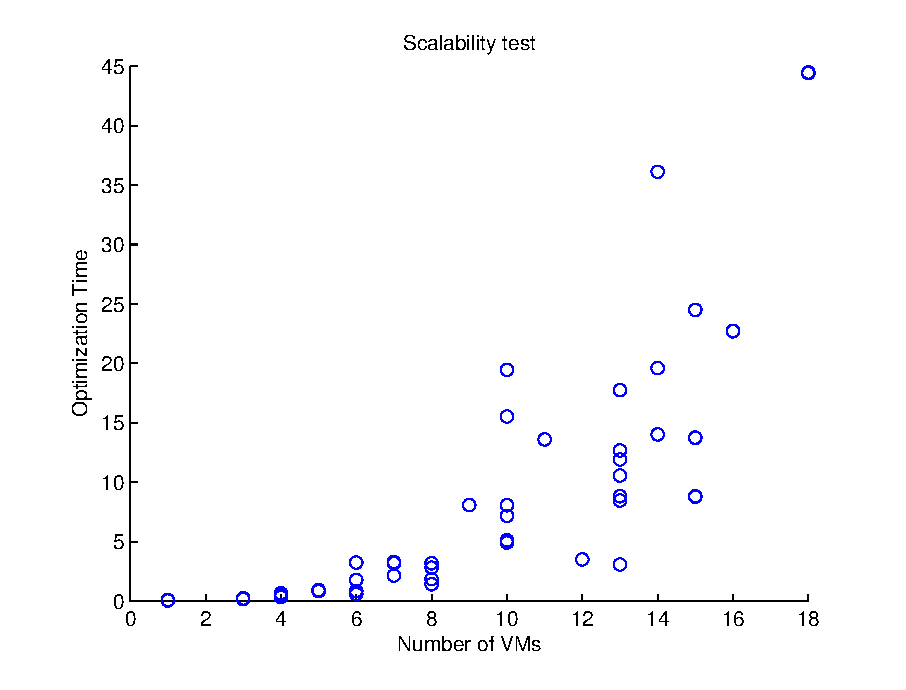
\includegraphics[width=0.8\textwidth]{image/centralized1/scalability}		
	%\caption{The relationship between the number of simulated VMs and the optimization time for each optimization step.}%
	%\label{fig:scalability} 
%\end{figure}

\section{Summary}  
\label{sec:future-work}
The purpose of this chapter was to demonstrate the advantage of ``adaptive empirical'' models relative to ``static empirical'' models in resource management.  
We investigated dynamic tuning of empirical resource allocation models. 
We described an approach which dynamically updates an empirical model for each application at runtime in order to capture the effects not considered in the initial specification of the model. 
This dynamic updating results in more accurate estimates being passed to the optimizer, allowing for better resource utilization on a global scale.  
We traced the effect of this tuning, in the overall system performance. We showed, in terms of performance, dynamic adjustment of model parameters using an EKF, can outperform a model built off-line using a non-linear regression. 

% We also investigated the model based optimization of resource shares in a private cloud where applications are distributed across a set of PMs. The goal was minimizing the SLA violations. While we focused only on the response time, considering other service level objectives would not change the approach (just the complexity of solving the optimization problem). 

% Future work will involve implementing the optimization algorithm in a distributed manner, in which applications interact in a peer-to-peer fashion to determine how much resource should be allocated to each. One can also investigate optimizing the dual optimization problem, which is more suitable for mapping to an agent-oriented optimization approach (see \cite{huang_macroeconomics_2008,izakian_auction_2010}).


